\documentclass[a4paper,11pt]{article}

\usepackage[english]{babel}
\usepackage[utf8]{inputenc}
\usepackage{graphicx}
\usepackage{caption}
\usepackage{subcaption}
\usepackage[T1]{fontenc}
\usepackage{setspace}
\usepackage{geometry}
\usepackage{titling}
\usepackage{float}
\usepackage{comment}
\usepackage[backend=biber]{biblatex}
\addbibresource{refs.bib}
\usepackage{lipsum}
\usepackage{tabularx,booktabs}
\newcolumntype{C}{>{\centering\arraybackslash}X} % centered version of "X" type
\setlength{\extrarowheight}{1pt}
\usepackage[compact]{titlesec}
\titlespacing*{\title}{0pt}{*1}{*1}
%\usepackage{savetrees}
 \geometry{
 a4paper,
 total={170mm,257mm},
 left=20mm,
 top=20mm,
 right=20mm,
 bottom=20mm,
 }
\title{\normalsize\textbf{Fault Tolerance Capabilities of Three, Four and Six Phase Configurations of a 24 Slot Modular PMSM}}
\date{}
\titlespacing\section{0pt}{11pt plus 4pt minus 2pt}{0pt plus 2pt minus 2pt}
\titlespacing\subsection{0pt}{11pt plus 4pt minus 2pt}{0pt plus 2pt minus 2pt}
\titlespacing\subsubsection{0pt}{11pt plus 4pt minus 2pt}{0pt plus 2pt minus 2pt}
\begin{document}
\vspace{-45mm}
\maketitle
\vspace{-23mm}

\textit{\normalsize\textbf{Abstract:}}
\textit{In this study, fault tolerance and redundancy capabilities of different phase and winding configurations of an Integrated Modular Motor Drive (IMMD) system is investigated. This is possible by manipulating gate drive signals of the inverter and end winding connections, without making any changes on the stator side of the electric machine. Three, four, symmetric and asymmetric six-phase topologies are described. Control strategies and redundancy possibilities of these different topologies under an open circuit fault condition are examined in MATLAB/Simulink environment and validated with Finite Element Analysis (FEA) software ANSYS/Maxwell. }

\section{\normalsize\textbf{Introduction}}
Integrated Modular Motor Drive (IMMD) is the concept of integrating power electronics, electric motor and other passive components of a drive to obtain a more compact system with higher power density compared to conventional motor drives \cite{immd-bible}. With the developments in safety-critical industrial applications, where IMMD concept would be quite related concerning efficiency and compactness, fault tolerance, reliability and redundancy of electric motor drive systems have become more important. This study examines assets and drawbacks of different phase configurations of the machine of an IMMD system, by means of redundancy and fault tolerance. 

\section{\normalsize\textbf{Design Specifications of IMMD System}}
For the machine topology, fractional slot concentrated winding (FSCW) permanent magnet synchronous motor (PMSM) is more suitable due to high power density and high efficiency advantages. Furthermore, complete (electric and physical) isolation of phases and achieving higher number of phases in FSCW increases the fault tolerance capability of the machine \cite{fscw}. Besides, integration of drive unit onto the FSCW machine \cite{mesutto} provides modularity for both machine and driver side, which brings redundant operation opportunity. In Figure \ref{fig:8kw}, one module of the driver, stator laminations and designed final product are presented. Main design specifications of the machine is given in Table \ref{specs}.

\begin{table*}[ht!]
\centering
 \caption{Design Specifications of IMMD}
\label{specs}
\begin{tabularx}{\textwidth}{@{}l*{10}{C}c@{}}

\toprule
Specification  &  Value & Specification  &  Value \\ 
\midrule
Rated Output Power & 8.5 kW & Speed & 600 rpm\\ 
Number of Slots ($Q_s$) & 24 & Pole Number (2p) & 20 \\
Stator Outer Diameter & 270 mm & Stack Length & 135 mm \\
DC Bus Voltage (Per Module) & 270 Vdc & & \\

\bottomrule
\end{tabularx}
\end{table*}

\begin{figure}[ht!]
\begin{subfigure}[b]{0.33\textwidth}
    \centering
    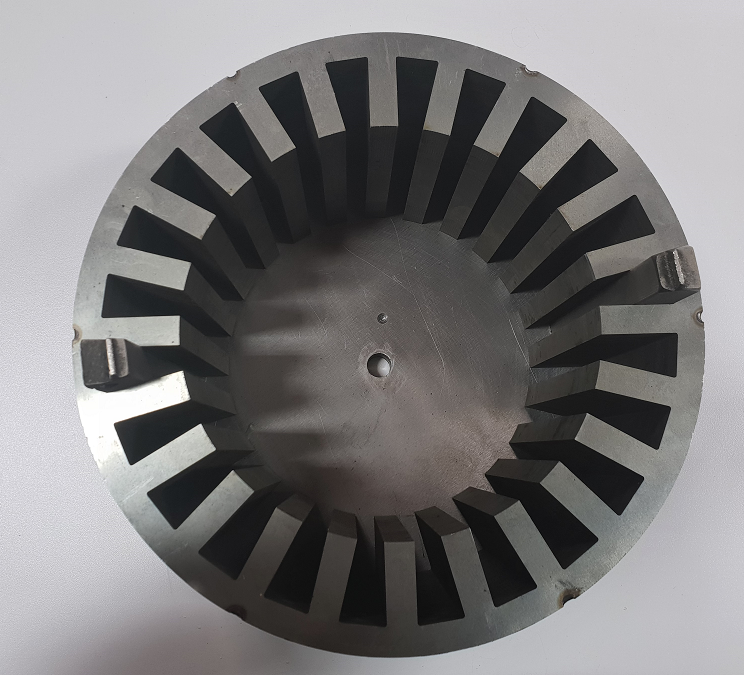
\includegraphics[width=\linewidth]{stator.png}
    \caption{24 Slot Stator}
    \label{fig:4phmmf}    
\end{subfigure}
\begin{subfigure}[b]{0.33\textwidth}
    \centering
    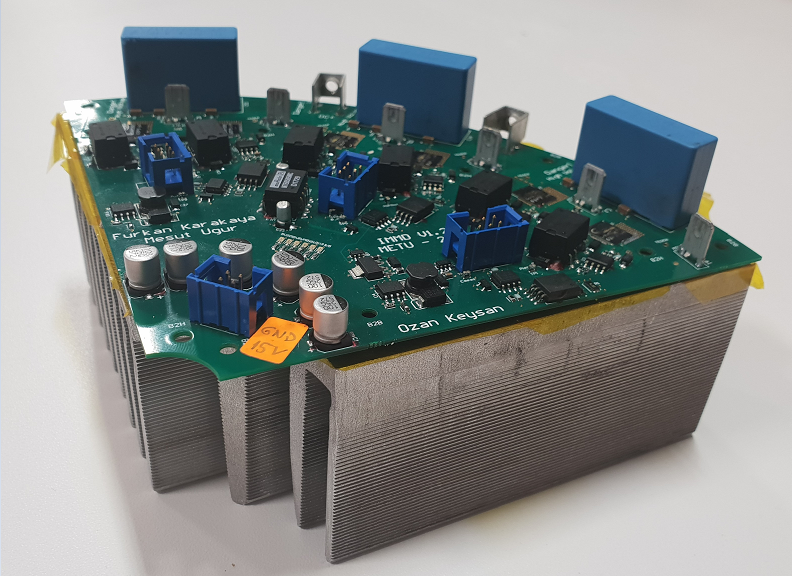
\includegraphics[width=\linewidth]{heatsink.png}
    \caption{Heatsink and Driver of a Module}
    \label{fig:s6phmmf}    
\end{subfigure}
\begin{subfigure}[b]{0.33\textwidth}
    \centering
    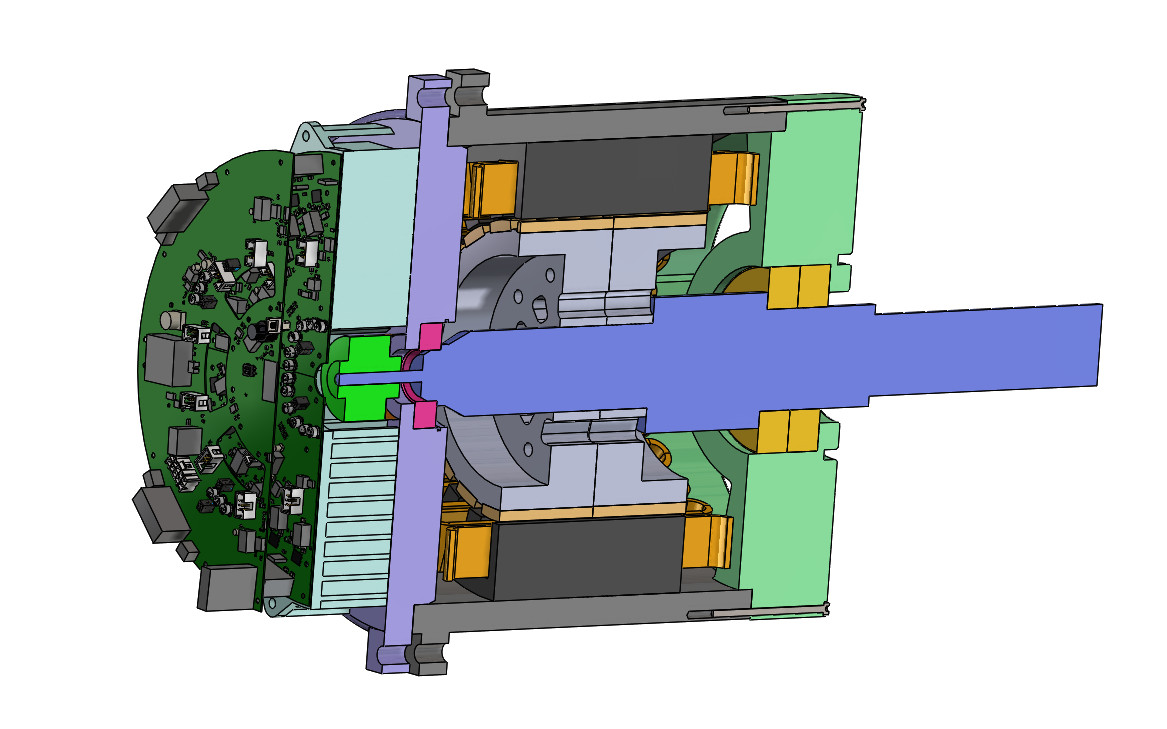
\includegraphics[width=\linewidth]{immd_csview.PNG}
    \caption{Cross-sectional View of IMMD}
    \label{fig:as6phmmf}    
\end{subfigure}
 \caption{8.5 kW IMMD System}
 \label{fig:8kw}
\end{figure}


\section{\normalsize\textbf{Three, Four and Six-Phase Winding Configurations}}
In a single phase fault condition, a star-connected three-phase machine is unable to operate as the machine cannot produce rotating MMF. For that reason, three-phase machines with a redundant phase leg or multiphase machines are more suitable for fault tolerant applications \cite{phaseleg}.
In this section, different configuration possibilities are to be evaluated. As the stator slot number ($Q_s$) is 24, three, four and six phase topologies are suitable to compare.\par
Figure \ref{fig:windings} presents possible winding diagrams for different phase numbers. As a result of pole-slot number combination, primary winding factors of three and six-phase topologies ($k_{w(1)} = 0.934$) are far better compared to four-phase topology ($k_{w(1)} = 0.880$). Furthermore, as given in Figure \ref{fig:harmonics}, four-phase topology introduces high number of MMF space harmonics. Among all of them, asymmetric six phase nearly eliminates all sub-harmonics, but due to its winding configuration, one of the phase inductances is expected to be lower than the others.


\begin{figure}[ht!]
\begin{subfigure}[b]{0.24\textwidth}
    \centering
    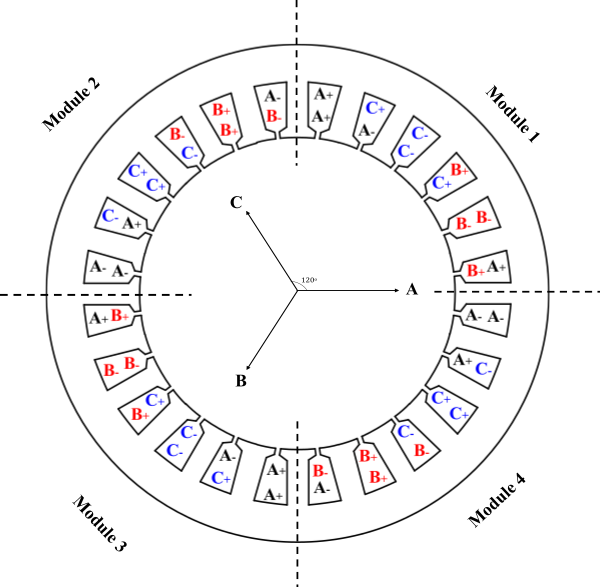
\includegraphics[width=\linewidth]{3ph.png}
    \caption{Three-Phase}
    \label{fig:3ph}    
\end{subfigure}
\begin{subfigure}[b]{0.24\textwidth}
    \centering
    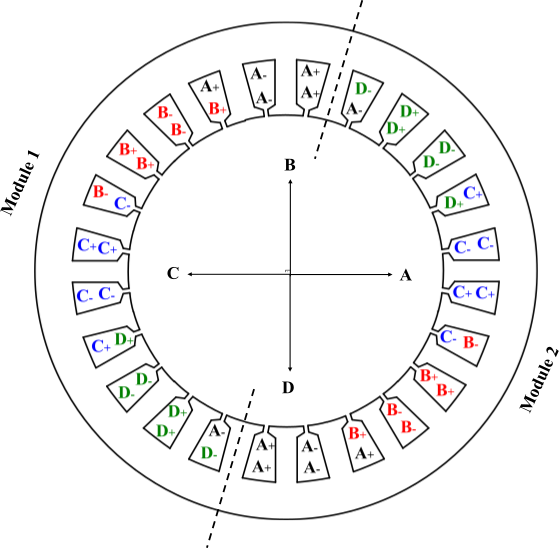
\includegraphics[width=\linewidth]{4ph.png}
    \caption{Four-Phase}
    \label{fig:4ph}    
\end{subfigure}
\begin{subfigure}[b]{0.24\textwidth}
    \centering
    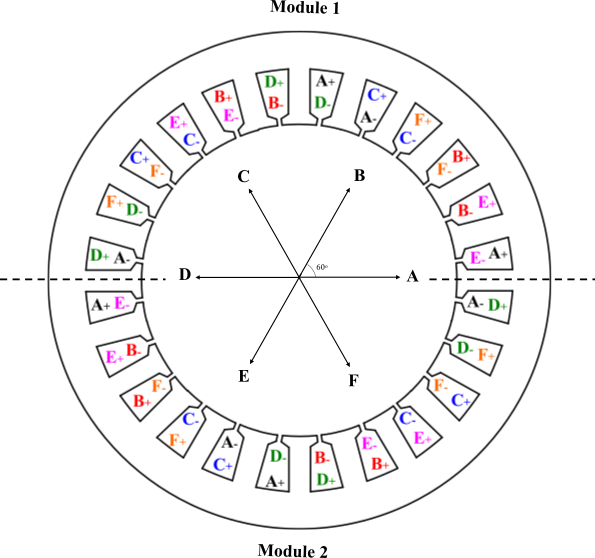
\includegraphics[width=\linewidth]{sym6ph.png}
    \caption{Symmetric Six-Phase}
    \label{fig:s6ph}    
\end{subfigure}
\begin{subfigure}[b]{0.24\textwidth}
    \centering
    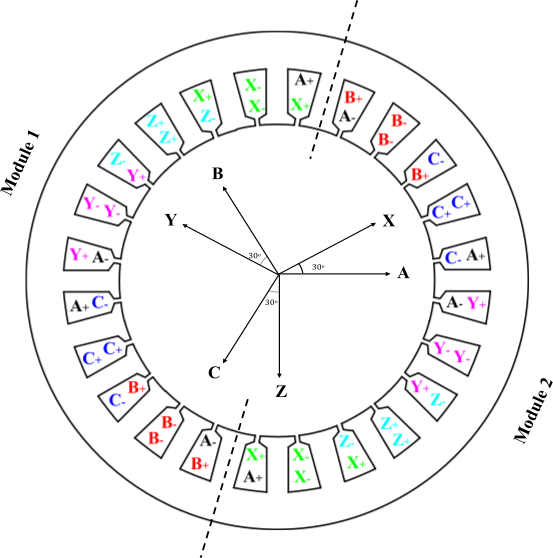
\includegraphics[width=\linewidth]{asym6ph.png}
    \caption{Asymmetric Six-Phase}
    \label{fig:as6ph}    
\end{subfigure}
 \caption{Winding Configurations}
 \label{fig:windings}
\end{figure}

\begin{figure}[ht!]
\begin{subfigure}[b]{0.33\textwidth}
    \centering
    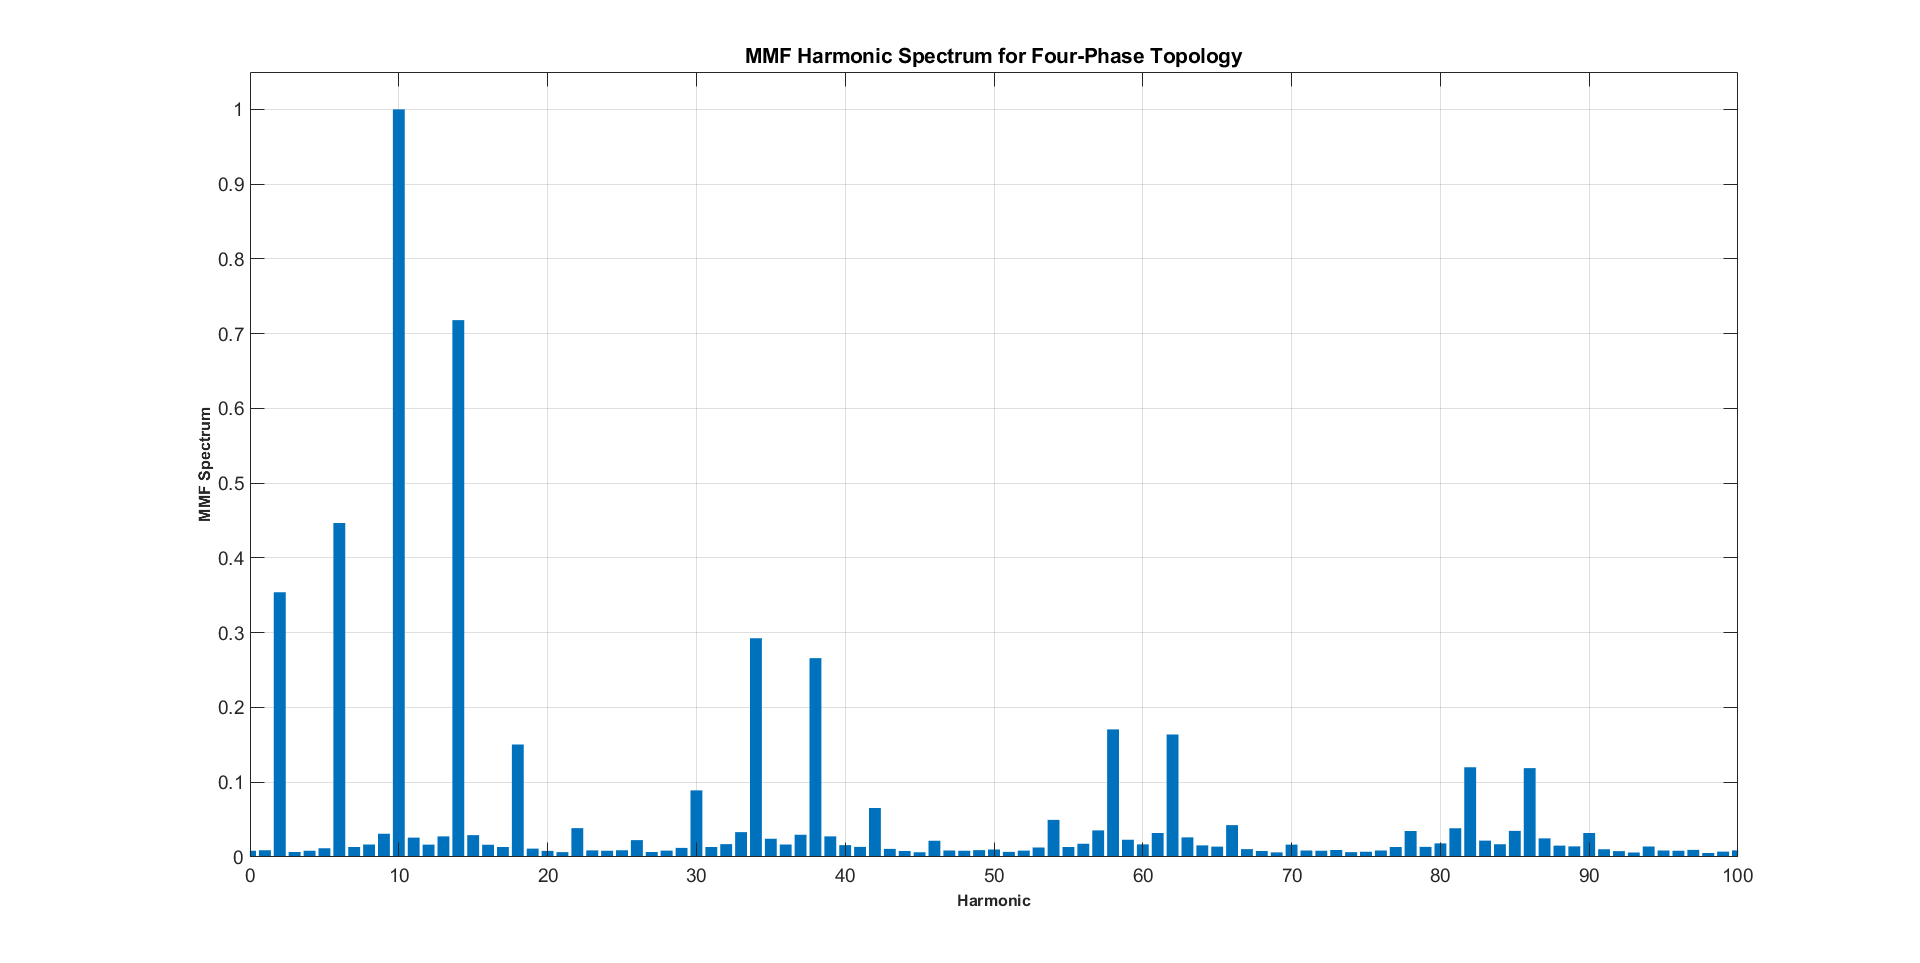
\includegraphics[width=\linewidth]{mmf_harm_4ph.png}
    \caption{Four-Phase}
    \label{fig:4phmmf}    
\end{subfigure}
\begin{subfigure}[b]{0.33\textwidth}
    \centering
    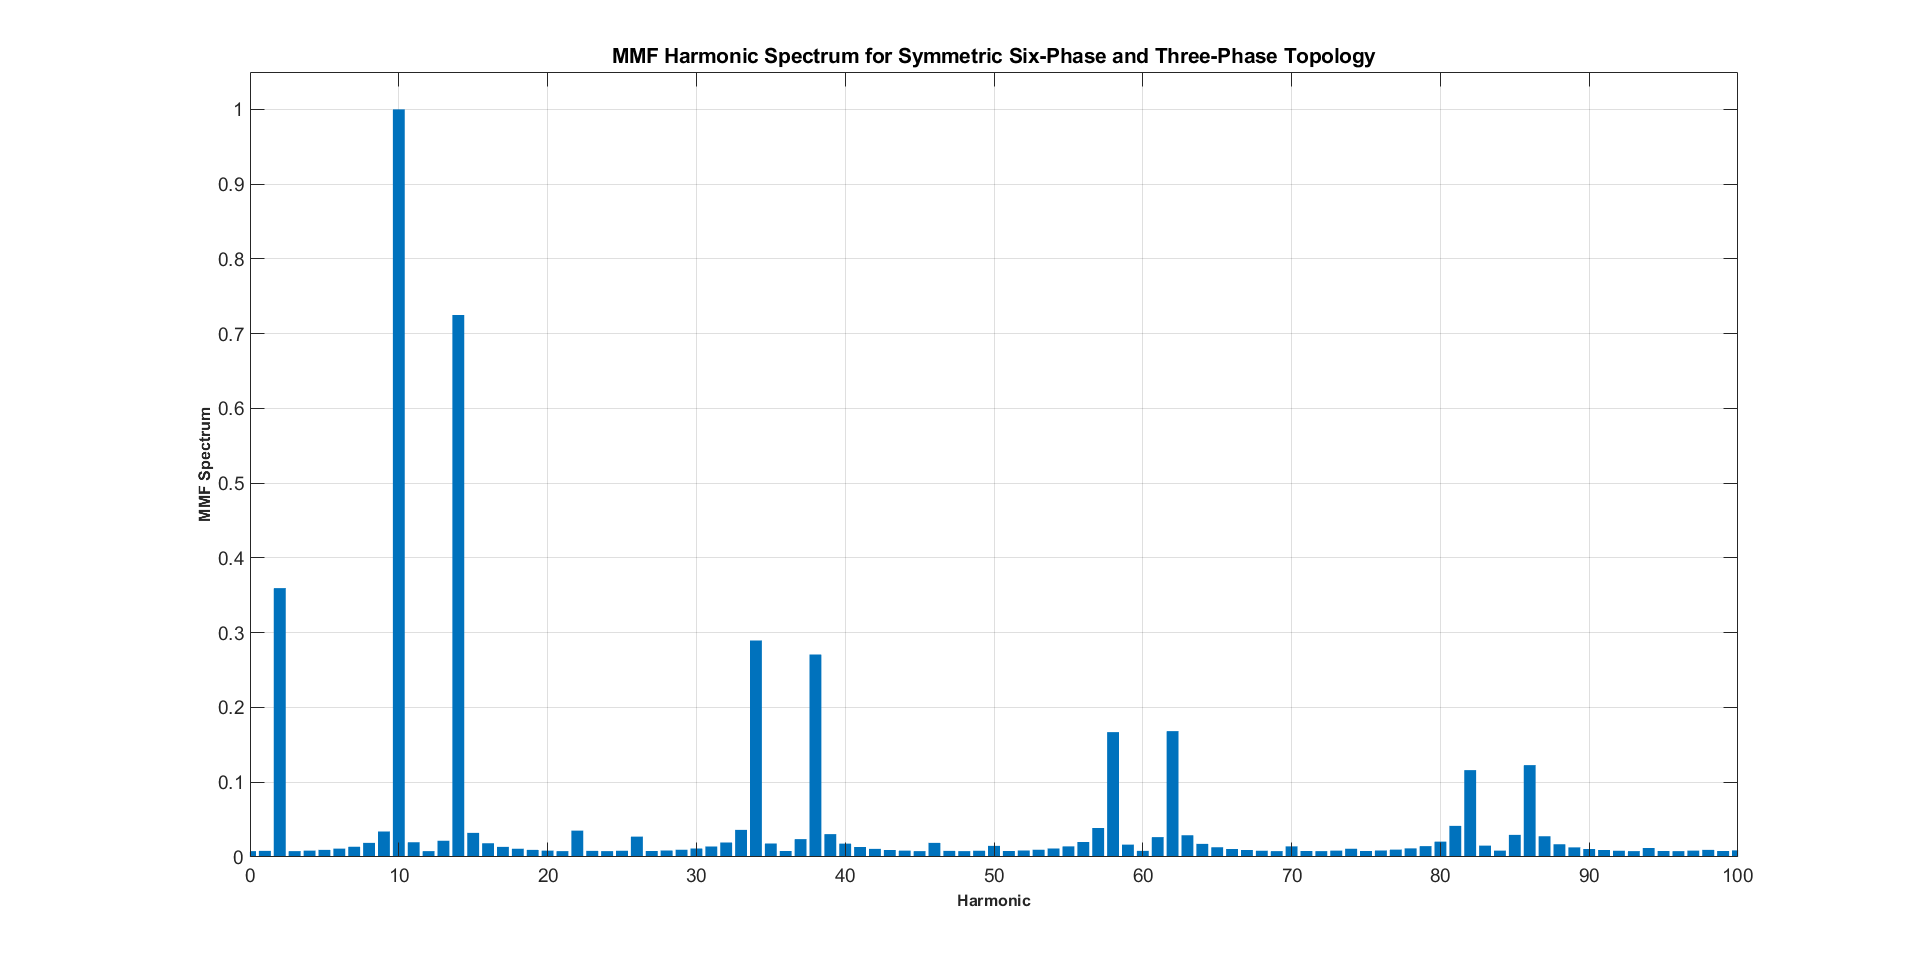
\includegraphics[width=\linewidth]{mmf_harm_sym.png}
    \caption{Symmetric Six-Phase}
    \label{fig:s6phmmf}    
\end{subfigure}
\begin{subfigure}[b]{0.33\textwidth}
    \centering
    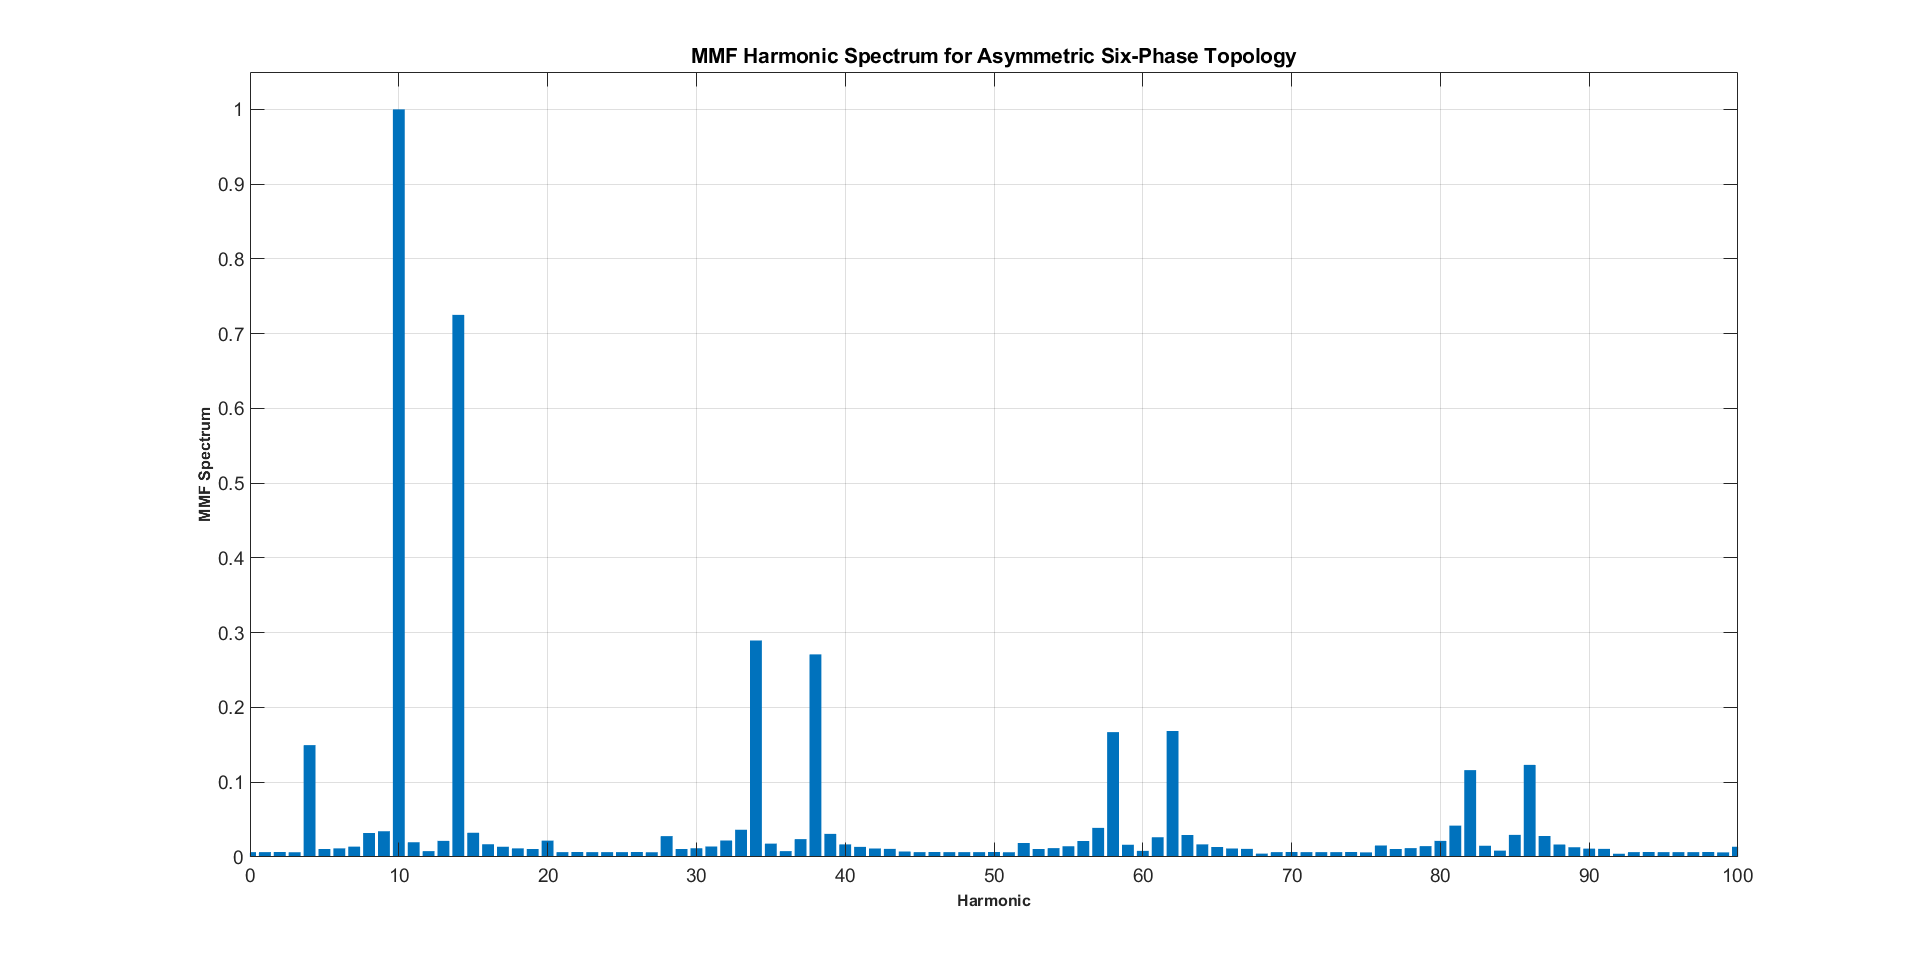
\includegraphics[width=\linewidth]{mmf_harm_asym.png}
    \caption{Asymmetric Six-Phase}
    \label{fig:as6phmmf}    
\end{subfigure}
 \caption{MMF Harmonic Spectrums}
 \label{fig:harmonics}
\end{figure}


\section{\normalsize\textbf{Comparison of Different Topologies}}
\subsection{\normalsize\textbf{Redundancy}}
As mentioned in the previous section, a three-phase machine is unable to operate properly under an open circuit failure (OCF) condition, as two phases cannot produce a rotating MMF. Accordingly, for the three-phase four module topology, OCF of a single phase results in turning off one module completely. In this case, output power is decreased by 25\%. Although symmetric six-phase topology has the same magnetic equivalent circuit with three-phase four module, neutral node connection between two modules in this topology provides multiphase operation opportunity and as a result, completely turning off one module is not necessary. Similar advantages are also applicable for four-phase and asymmetric six-phase cases. \par
On the other hand, decreasing the module number by half brings out other drawbacks. In a controller fault situation, which affects one module of the driver, decreases the motor output power to half, where it only decreases a quarter in initially proposed three-phase four module IMMD structure.

\subsection{\normalsize\textbf{Open Circuit Failure (OCF) Responses and Recovery}}

To examine the fault tolerance capability of the different configurations, winding OCF responses and corresponding recovery techniques have been reviewed. The major advantage of multiphase machines under this condition is maintaining proper operation and producing same rotating MMF by manipulating current phasors of remaining phases. Although this can be achieved in several ways, the most convenient recovery option is the one where adjusted current values exceed rated current the least.\par
For symmetric six-phase topology, in the absence of phase A current of one module, magnitude of current phasors have been increased by 30\% of its rated value in order to produce same rotating MMF, where their phases have been shifted -35.04, -6, 0, 6 and 35.04 degrees with respect to their initial phases in counter clockwise direction, respectively \cite{recover} (Further details of these calculations and recovery techniques will be provided in full paper.). Simulation results obtained in MATLAB/Simulink for normal, faulted and recovered operation of symmetric six-phase topology is given in \ref{fig:ocfresponse}. In contrast to faulted operation, torque ripple at steady state decreased with modified phasors, as expected. Simulation results of other configurations will be presented in full paper.


\begin{figure}[ht!]
\begin{subfigure}[b]{0.33\textwidth}
    \centering
    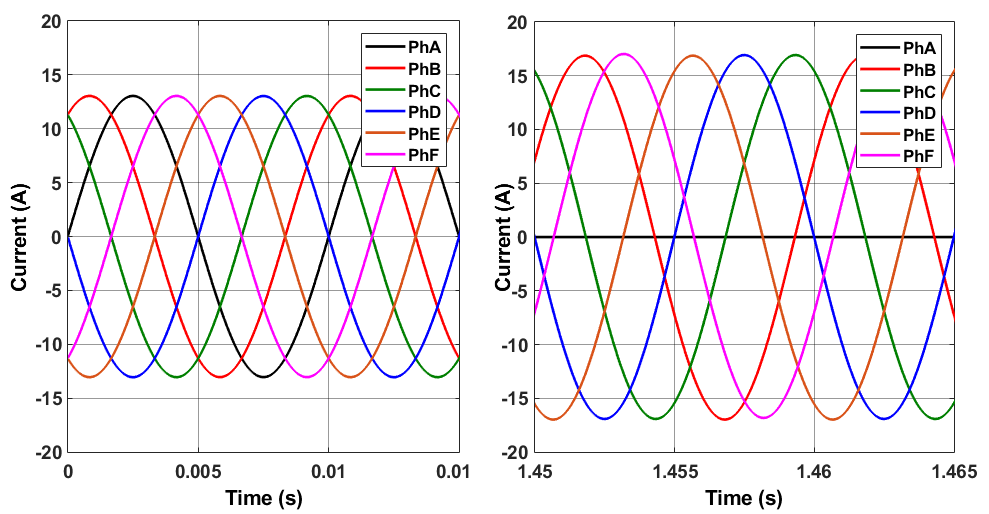
\includegraphics[width=\linewidth]{c1.png}
    \caption{Phase Currents}
    \label{fig:ocfcurrent}    
\end{subfigure}
\begin{subfigure}[b]{0.33\textwidth}
    \centering
    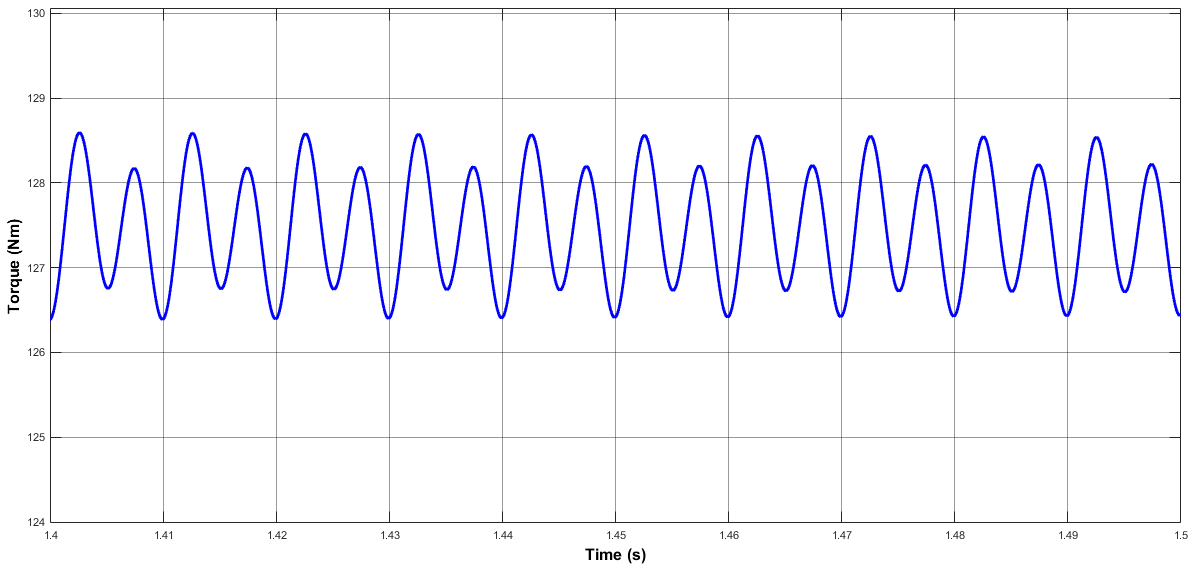
\includegraphics[width=\linewidth]{ss_recover_torque.png}
    \caption{Torque Ripple (with Simulink)}
    \label{fig:ocftorque}    
\end{subfigure}
\begin{subfigure}[b]{0.33\textwidth}
    \centering
    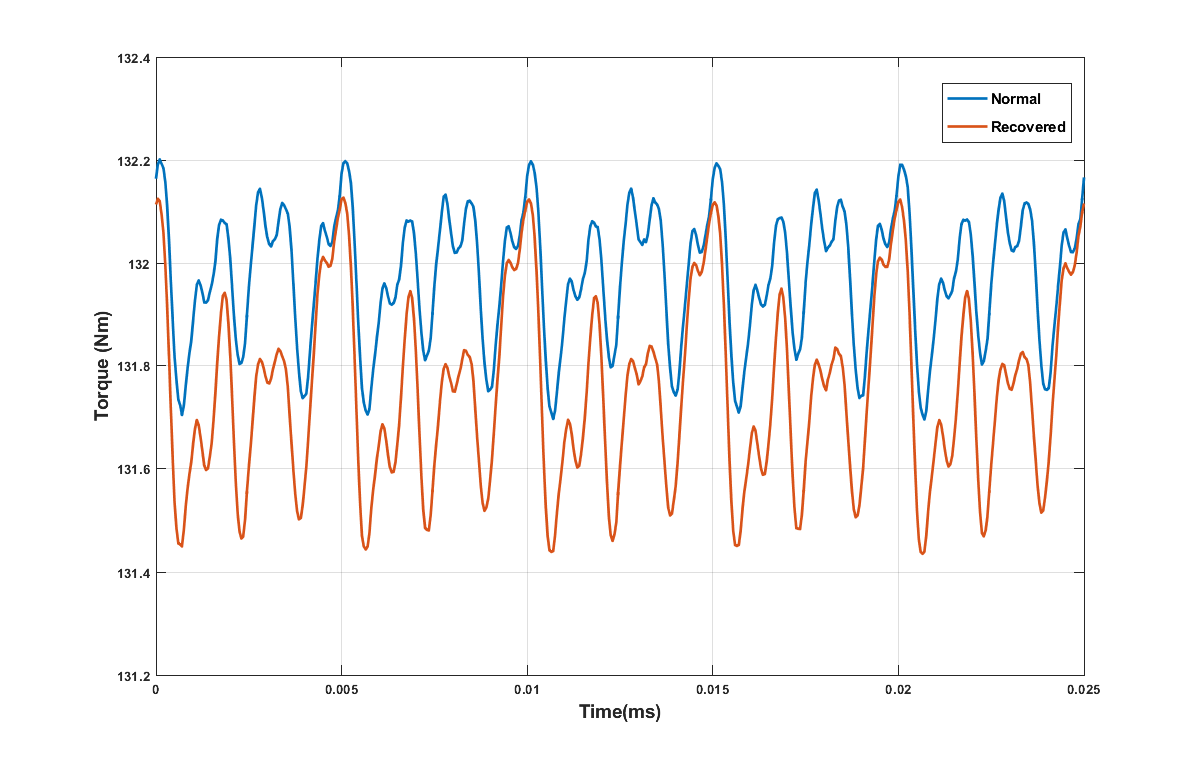
\includegraphics[width=\linewidth]{ss_recover_torque_fea2.png}
    \caption{Torque Ripple (with FEA)}
    \label{fig:ocftorquefea}   
\end{subfigure}
 \caption{Normal and OCF Recovered Steady State Operation of Symmetric Six-Phase Machine}
 \label{fig:ocfresponse}
\end{figure}

\section{\normalsize\textbf{Conclusions and Future Work}}
This paper compared assets and disadvantages of three, four and six phase configurations of the machine of an IMMD by means of fault tolerance. These have been summarized briefly in Table \ref{compare}. In full paper, simulation results for all configurations, further comparison criterion and analytical verification of fault recovery method are to be added and explained in detail.

\begin{table*}[ht!]
 \caption{Comparison of Different Topologies}
\label{kd}
\begin{tabularx}{\textwidth}{@{}l*{10}{C}c@{}}
\toprule
Advantages      & Three-Phase  & Four-Phase & Symmetric Six-Phase & Asymmetric Six-Phase \\ 
\midrule
Redundancy Factor    & low    & medium    & high   & high \\ 
Overcurrent in OCF   & medium    & high  & low    & low \\ 
Inductance Balance  &  high &   high &    high &  low\\
MMF Harmonics  & medium    & high  & medium  & low  \\ 


\bottomrule
\end{tabularx}
\label{compare}
\end{table*}

\AtNextBibliography{\tiny}
\printbibliography

\end{document}
